\documentclass{beamer}
\usetheme{metropolis}           % Use metropolis theme

\usepackage[T2A]{fontenc}
\usepackage[utf8]{inputenc}
\usepackage[english, main=russian]{babel}

\usepackage{listingsutf8}
\usepackage[ruled]{algorithm}
\usepackage{algorithmicx}
\usepackage[noend]{algpseudocode}
\usepackage{amsmath}
\usepackage{caption}
\usepackage{graphicx}
\usepackage{subcaption}
\usepackage{float}

\usepackage{tikz}
\usetikzlibrary{shapes.misc}
\usetikzlibrary{trees}

\floatname{algorithm}{Листинг}
\renewcommand{\algorithmname}{Листинг}

\title{Сравнение методов коммуникации между процессами в среде Linux}
\date{\today} \author{Старовойтов Александр} \author[me]{Выполнил: Старовойтов Александр
  ИУ9-51Б\\[1mm]Руководитель: Цалкович П.А.}
% \thanks
% \institute{МГТУ им. Н.Э. Баумана}
\begin{document}
\maketitle

\begin{frame}{Цели и задачи}
  \metroset{block=fill}
	\begin{alertblock}{Цель}
		Провести сравнительный анализ механизмов межпроцессной коммуникации в Linux.
	\end{alertblock}
	\begin{alertblock}{Задачи}
		\begin{itemize}
			\item Изучить методы межпроцессной коммуникации;
			\item Реализовать библиотеку для их поддержки на C++;
			\item Реализовать бенчмарки;
			\item Собрать данные о производительности и проанализировать;
		\end{itemize}
	\end{alertblock}
\end{frame}

\begin{frame}{Определение межпроцессной коммуникации}

\textbf{Межпроцессное взаимодействие} --- это обмен данными между потоками разных
процессов, реалзизованный с помощью механизмов
предоставляемых операционной системой.

\end{frame}

\begin{frame}{Классификация методов межпроцессной коммуникации}

  \begin{itemize}
	\item \textbf{Коммуникационные}: фокусируются на
	обмене данными между процессами;
	\item \textbf{Синхронизационные}: для синхронизации действий между различными
	процессами;
	\item \textbf{Сигналы}: могут использоваться как для обмена данными, так и для
	синхронизации.
  \end{itemize}

\end{frame}

\begin{frame}{Коммуникационные методы}

\begin{figure}[H]
  \centering
  \begin{minipage}[t]{\textwidth}
    \centering
    \begin{tikzpicture}[grow'=right,
      every node/.style={shape=rectangle,draw,align=center}]
      \node {Коммуникационные\\механизмы}
      [level distance=50mm, sibling distance=40mm, edge from parent fork right]
        child {
          node {Передача данных}
        }
        child {
          node {Разделяемая память}
        };
    \end{tikzpicture}
  \end{minipage}
  \caption{Классификация коммуникационных механизмов межпроцессного взаимодействия в Linux.}
  \label{fig:communication_ipc_taxonomy}
\end{figure}

\end{frame}

\begin{frame}{Передача данных}

\begin{figure}[H]
  \centering
  \begin{minipage}[t]{\textwidth}
    \centering
	\resizebox{0.7\textwidth}{7cm}{%
    \begin{tikzpicture}[grow'=right,
      every node/.style={shape=rectangle,draw,align=center}]
          \node {Передача\\данных}
          [level distance=45mm, sibling distance=30mm, edge from parent fork right]
            child {
              node {Поток байтов}
              [shape=rounded rectangle, level distance=40mm, sibling distance=10mm, edge from parent fork right]
                child {
                  node [shape=rounded rectangle] {Каналы}
                }
                child {
                  node [shape=rounded rectangle] {FIFO}
                }
                child {
                  node [shape=rounded rectangle, yshift=-3mm] {Потоковые\\сокеты}
                }
            }
            child {
              node [shape=rounded rectangle] {Псевдо-\\терминал}
            }
            child {
              node {Сообщения}
              [level distance=40mm, sibling distance=25mm, edge from parent fork right]
                child {
                  node [shape=rounded rectangle] {Очереди\\сообщений\\System V}
                }
                child {
                  node [shape=rounded rectangle] {Очереди\\сообщений\\POSIX}
                }
                child {
                  node [shape=rounded rectangle] {Датаграммные\\сокеты}
                }
        };
    \end{tikzpicture}
	}
  \end{minipage}
  \caption{Классификация методов передачи данных.}
  \label{fig:data_flow}
\end{figure}

\end{frame}

\begin{frame}{Разделяемая память}

\begin{figure}[H]
  \centering
  \begin{minipage}[t]{\textwidth}
    \centering
	\resizebox{\textwidth}{7cm}{%
    \begin{tikzpicture}[grow'=right,
      every node/.style={shape=rectangle,draw,align=center}]
	  \node {Разделяемая\\память} [level distance=45mm, sibling distance=25mm, edge from parent fork right]
          child {
            node [shape=rounded rectangle, xshift=15mm] {Разделяемая память System V}
          }
          child {
            node [shape=rounded rectangle, xshift=13mm] {Разделяемая память POSIX}
          }
          child {
            node {Отображаемая\\память}
            [level distance=45mm, sibling distance=25mm, edge from parent fork right]
              child {
                node [shape=rounded rectangle] {Анонимное\\отображение}
              }
              child {
                node [shape=rounded rectangle] {Отображение\\файла}
              }
          };
    \end{tikzpicture}
	}
  \end{minipage}
  \caption{Классификация разделяемой памяти.}
  \label{fig:memory_mapping}
\end{figure}

\end{frame}

\begin{frame}{Архитектура библиотеки}

\begin{figure}[H]
  \centering
  \begin{minipage}[t]{\textwidth}
    \centering
    \resizebox{\textwidth}{6cm}{%
    % generated by Plantuml 1.2024.4
\definecolor{plantucolor0000}{RGB}{241,241,241}
\definecolor{plantucolor0001}{RGB}{24,24,24}
\definecolor{plantucolor0002}{RGB}{173,209,178}
\definecolor{plantucolor0003}{RGB}{0,0,0}
\definecolor{plantucolor0004}{RGB}{180,167,229}
\begin{tikzpicture}[yscale=-1
,pstyle0/.style={color=plantucolor0001,fill=plantucolor0000,line width=0.5pt}
,pstyle1/.style={color=plantucolor0001,fill=plantucolor0002,line width=1.0pt}
,pstyle2/.style={color=plantucolor0001,line width=0.5pt}
,pstyle3/.style={color=plantucolor0001,fill=plantucolor0004,line width=1.0pt}
,pstyle4/.style={color=plantucolor0001,line width=1.0pt}
,pstyle5/.style={color=plantucolor0001,fill=plantucolor0001,line width=1.0pt}
]
\draw[pstyle0] (7pt,12pt) arc (180:270:5pt) -- (12pt,7pt) -- (593.3049pt,7pt) arc (270:360:5pt) -- (598.3049pt,12pt) -- (598.3049pt,82.5938pt) arc (0:90:5pt) -- (593.3049pt,87.5938pt) -- (12pt,87.5938pt) arc (90:180:5pt) -- (7pt,82.5938pt) -- cycle;
\draw[pstyle1] (253.358pt,23pt) ellipse (11pt and 11pt);
\node at (253.358pt,23pt)[]{\textbf{\Large C}};
\node at (273.858pt,14.8516pt)[below right,color=black]{Subprocess};
\draw[pstyle2] (8pt,39pt) -- (597.3049pt,39pt);
\node at (13pt,43pt)[below right,color=black]{StreamBuf stdout};
\draw[pstyle2] (8pt,63.2969pt) -- (597.3049pt,63.2969pt);
\node at (13pt,67.2969pt)[below right,color=black]{Subprocess(std::function\textless void(Streambuf stdin)\textgreater  childProgram, RWIpc)};
\draw[pstyle0] (572.5pt,169.59pt) arc (180:270:5pt) -- (577.5pt,164.59pt) -- (687.8053pt,164.59pt) arc (270:360:5pt) -- (692.8053pt,169.59pt) -- (692.8053pt,207.59pt) arc (0:90:5pt) -- (687.8053pt,212.59pt) -- (577.5pt,212.59pt) arc (90:180:5pt) -- (572.5pt,207.59pt) -- cycle;
\draw[pstyle3] (587.5pt,180.59pt) ellipse (11pt and 11pt);
\node at (587.5pt,180.59pt)[]{\textbf{\Large I}};
\node at (601.5pt,172.4416pt)[below right,color=black]{\textit{StreamBuf}};
\draw[pstyle2] (573.5pt,196.59pt) -- (691.8053pt,196.59pt);
\draw[pstyle2] (573.5pt,204.59pt) -- (691.8053pt,204.59pt);
\draw[pstyle0] (259.31pt,169.59pt) arc (180:270:5pt) -- (264.31pt,164.59pt) -- (340.9933pt,164.59pt) arc (270:360:5pt) -- (345.9933pt,169.59pt) -- (345.9933pt,207.59pt) arc (0:90:5pt) -- (340.9933pt,212.59pt) -- (264.31pt,212.59pt) arc (90:180:5pt) -- (259.31pt,207.59pt) -- cycle;
\draw[pstyle3] (274.31pt,180.59pt) ellipse (11pt and 11pt);
\node at (274.31pt,180.59pt)[]{\textbf{\Large I}};
\node at (288.31pt,172.4416pt)[below right,color=black]{\textit{RWIpc}};
\draw[pstyle2] (260.31pt,196.59pt) -- (344.9933pt,196.59pt);
\draw[pstyle2] (260.31pt,204.59pt) -- (344.9933pt,204.59pt);
\draw[pstyle0] (201.91pt,278.59pt) arc (180:270:5pt) -- (206.91pt,273.59pt) -- (398.3992pt,273.59pt) arc (270:360:5pt) -- (403.3992pt,278.59pt) -- (403.3992pt,381.7775pt) arc (0:90:5pt) -- (398.3992pt,386.7775pt) -- (206.91pt,386.7775pt) arc (90:180:5pt) -- (201.91pt,381.7775pt) -- cycle;
\draw[pstyle1] (280.9659pt,289.59pt) ellipse (11pt and 11pt);
\node at (280.9659pt,289.59pt)[]{\textbf{\Large C}};
\node at (301.4659pt,281.4416pt)[below right,color=black]{Pipe};
\draw[pstyle2] (202.91pt,305.59pt) -- (402.3992pt,305.59pt);
\node at (207.91pt,309.59pt)[below right,color=black]{int fd};
\draw[pstyle2] (202.91pt,329.8869pt) -- (402.3992pt,329.8869pt);
\node at (207.91pt,333.8869pt)[below right,color=black]{Pipe()};
\node at (207.91pt,350.1838pt)[below right,color=black]{StreamBuf GetReader()};
\node at (207.91pt,366.4806pt)[below right,color=black]{StreamBuf GetWriter()};
\draw[pstyle0] (633.35pt,28.3pt) arc (180:270:5pt) -- (638.35pt,23.3pt) -- (774.9595pt,23.3pt) arc (270:360:5pt) -- (779.9595pt,28.3pt) -- (779.9595pt,66.3pt) arc (0:90:5pt) -- (774.9595pt,71.3pt) -- (638.35pt,71.3pt) arc (90:180:5pt) -- (633.35pt,66.3pt) -- cycle;
\draw[pstyle1] (648.35pt,39.3pt) ellipse (11pt and 11pt);
\node at (648.35pt,39.3pt)[]{\textbf{\Large C}};
\node at (662.35pt,31.1516pt)[below right,color=black]{std::streambuf};
\draw[pstyle2] (634.35pt,55.3pt) -- (778.9595pt,55.3pt);
\draw[pstyle2] (634.35pt,63.3pt) -- (778.9595pt,63.3pt);
\draw[pstyle0] (646.71pt,311.19pt) arc (180:270:5pt) -- (651.71pt,306.19pt) -- (753.5957pt,306.19pt) arc (270:360:5pt) -- (758.5957pt,311.19pt) -- (758.5957pt,349.19pt) arc (0:90:5pt) -- (753.5957pt,354.19pt) -- (651.71pt,354.19pt) arc (90:180:5pt) -- (646.71pt,349.19pt) -- cycle;
\draw[pstyle1] (661.71pt,322.19pt) ellipse (11pt and 11pt);
\node at (661.71pt,322.19pt)[]{\textbf{\Large C}};
\node at (675.71pt,314.0416pt)[below right,color=black]{FdBufOut};
\draw[pstyle2] (647.71pt,338.19pt) -- (757.5957pt,338.19pt);
\draw[pstyle2] (647.71pt,346.19pt) -- (757.5957pt,346.19pt);
\draw[pstyle0] (513.72pt,311.19pt) arc (180:270:5pt) -- (518.72pt,306.19pt) -- (606.5937pt,306.19pt) arc (270:360:5pt) -- (611.5937pt,311.19pt) -- (611.5937pt,349.19pt) arc (0:90:5pt) -- (606.5937pt,354.19pt) -- (518.72pt,354.19pt) arc (90:180:5pt) -- (513.72pt,349.19pt) -- cycle;
\draw[pstyle1] (528.72pt,322.19pt) ellipse (11pt and 11pt);
\node at (528.72pt,322.19pt)[]{\textbf{\Large C}};
\node at (542.72pt,314.0416pt)[below right,color=black]{FdBufIn};
\draw[pstyle2] (514.72pt,338.19pt) -- (610.5937pt,338.19pt);
\draw[pstyle2] (514.72pt,346.19pt) -- (610.5937pt,346.19pt);
\draw[pstyle4] (407.8358pt,92.6958pt) ..controls (466.1258pt,117.2958pt) and (527.94pt,143.39pt) .. (577.14pt,164.16pt);
\draw[pstyle5] (396.78pt,88.03pt) -- (400.7526pt,94.0482pt) -- (407.8358pt,92.6958pt) -- (403.8632pt,86.6777pt) -- (396.78pt,88.03pt) -- cycle;
\draw[pstyle4] (302.65pt,99.84pt) ..controls (302.65pt,124.45pt) and (302.65pt,143.28pt) .. (302.65pt,164.1pt);
\draw[pstyle5] (302.65pt,87.84pt) -- (298.65pt,93.84pt) -- (302.65pt,99.84pt) -- (306.65pt,93.84pt) -- (302.65pt,87.84pt) -- cycle;
\node at (303.65pt,118.59pt)[below right,color=black]{use};
\draw[pstyle4] (685.8245pt,87.5057pt) ..controls (672.1645pt,113.2157pt) and (658.75pt,138.46pt) .. (645.08pt,164.2pt);
\draw[pstyle4] (694.27pt,71.61pt) -- (680.5259pt,84.6905pt) -- (691.123pt,90.3209pt) -- (694.27pt,71.61pt) -- cycle;
\draw[pstyle4] (652.4373pt,229.0509pt) ..controls (665.3573pt,254.8209pt) and (677.96pt,279.95pt) .. (690.9pt,305.75pt);
\draw[pstyle4] (644.37pt,212.96pt) -- (647.0737pt,231.74pt) -- (657.801pt,226.3618pt) -- (644.37pt,212.96pt) -- cycle;
\draw[pstyle4] (612.8677pt,229.0484pt) ..controls (599.9377pt,254.8184pt) and (587.34pt,279.95pt) .. (574.41pt,305.75pt);
\draw[pstyle4] (620.94pt,212.96pt) -- (607.5049pt,226.3577pt) -- (618.2305pt,231.7392pt) -- (620.94pt,212.96pt) -- cycle;
\draw[pstyle4] (302.65pt,230.96pt) ..controls (302.65pt,247.41pt) and (302.65pt,252.17pt) .. (302.65pt,273.18pt);
\draw[pstyle4] (302.65pt,212.96pt) -- (296.65pt,230.96pt) -- (308.65pt,230.96pt) -- (302.65pt,212.96pt) -- cycle;
\end{tikzpicture}

    }
  \end{minipage}
  \caption{Диаграмма классов библиотеки.}
  \label{fig:classes}
\end{figure}

\end{frame}

\begin{frame}{Тестирование корректности}

  \begin{alertblock}{Для проверки корректности кода было применено:}
  \begin{itemize}
    \item Покрытие кода юнит-тестами;
    \item Санитайзеры;
	\item Статический анализатор clang-tidy;
	\item valgrind.
  \end{itemize}
  \end{alertblock}

\end{frame}

\begin{frame}{Реализация бенчмарков}

  \begin{alertblock}{Бенчмарки построены по одному шаблону:}
  \begin{itemize}
    \item Однонаправленная передача (от дочернего процесса к родительскому);
    \item 40'000 байт в одной итерации;
	\item Настраивается размер сообщения и их количество;
	\item fork() для создания дочернего процесса.
  \end{itemize}
  \end{alertblock}

\end{frame}

\begin{frame}{Результаты измерений производительности}

\begin{figure}[H]
  \centering
  \begin{minipage}[t]{\textwidth}
    \centering
    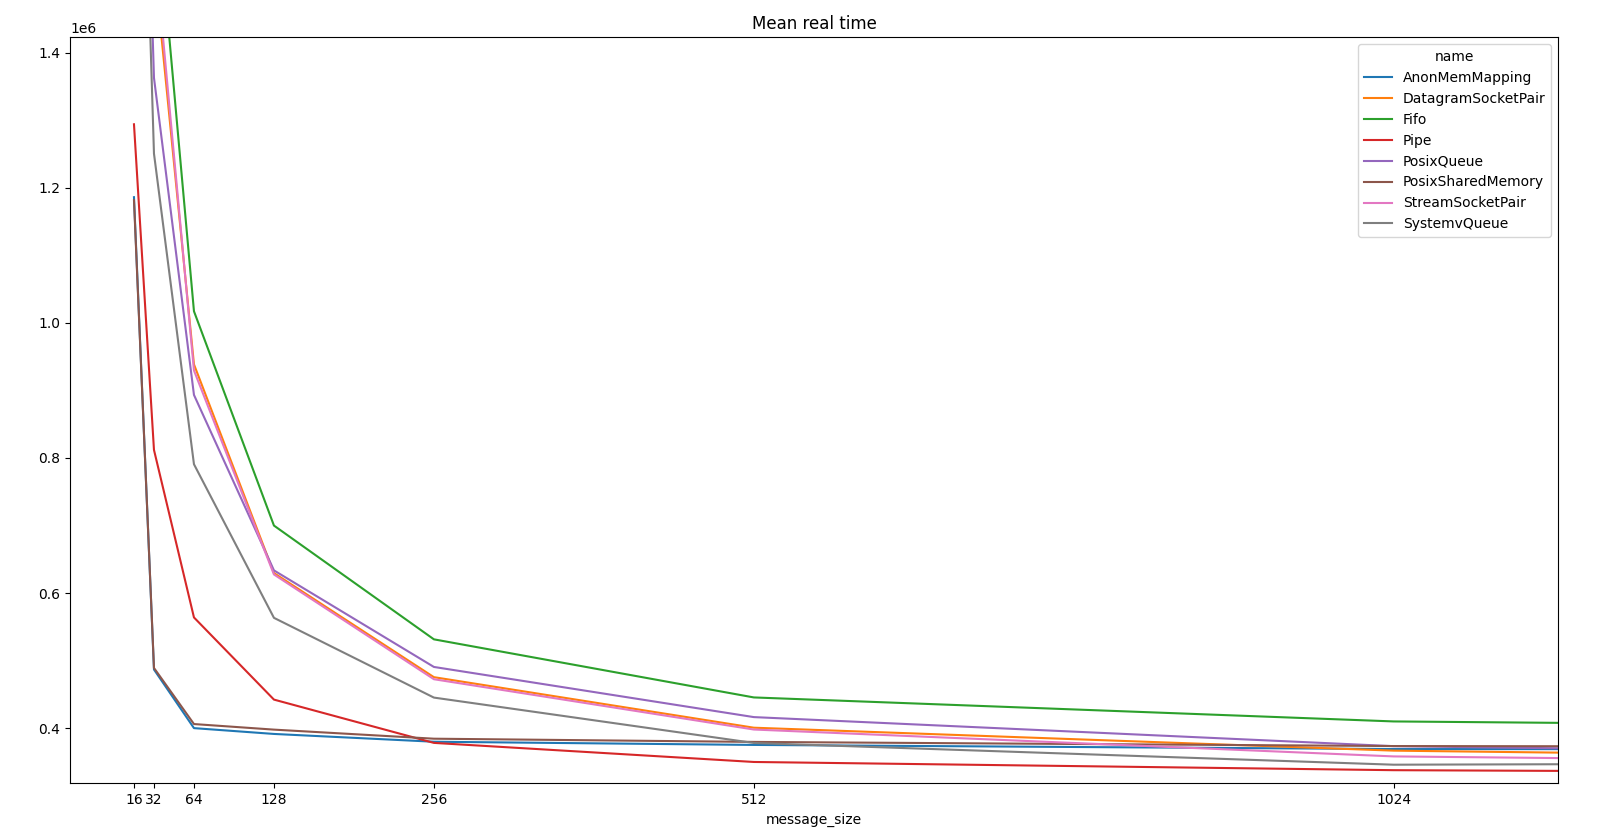
\includegraphics[width=\textwidth]{./imgs/performance.png}
  \end{minipage}
  \caption{Сравнительный график производительности средств межпроцессной
    коммуникации.}
  \label{fig:performance}
\end{figure}

\end{frame}

\begin{frame}{Заключение}
  \begin{alertblock}{Возможные улучшения}
  \begin{itemize}
    \item Тестирование и замеры производительности на других реализациях UNIX;
    \item Расширение интерфейсов для поддержки двунаправленной коммуникации.
  \end{itemize}
  \end{alertblock}
\end{frame}

\begin{frame}{Заключение}
  В ходе разработки были получены следующие навыки:
    \begin{itemize}
      \item Разработка программ с использованием межпроцессной коммуникации;
      \item Системное программирование на C++ в среде Linux;
      \item Реализация бенчмарков;
	  \item Анализ данных о производительности, их представление в виде
			графиков.
    \end{itemize}
\end{frame}

\end{document}
